\chapter{Systemarkitektur}
Dette kapitel har til formål at beskrive arkitekturen for WinePrep.

\section{BDD}
Det overordnede system er beskrevet på figur \ref{BDD_WinePrepPNG}. BDD'et viser WinePrep opdelt i tre underblokke: \textbf{Brugergrænseflade}, \textbf{Positionering} og \textbf{Åbningsmekanisme}.

\begin{figure}[H]
	\centerline{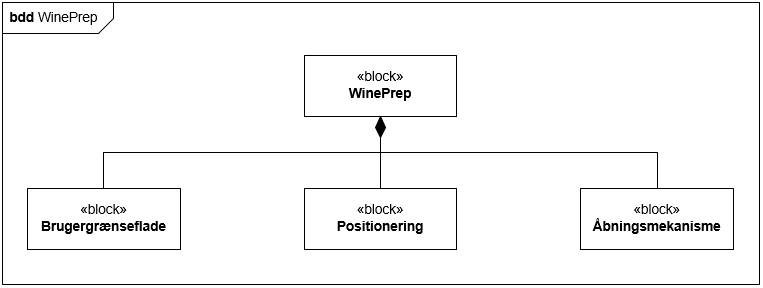
\includegraphics[scale=0.4]{Diagrammer/BDD_WinePrep.png}}
	\caption{BDD over WinePrep}
	\label{BDD_WinePrepPNG}
\end{figure}

\noindent\textbf{Brugergrænsefladen} betjenes af bruger og initierer usecasene som beskrevet i Krav (indsæt reference hertil).
\\
\\
\textbf{Positionering} finder vinflaskens position og flytter \textbf{Åbningsmekanismen}, så den er klar til at åbne vinflasken.
\\
\\
\textbf{Åbningsmekanismen} fjerner proppen fra flasken og dispenserer proppen.
\\
\\
For at forstå den interne funktionalitet og kompleksitet i blokkene \textbf{Positionering} og \textbf{Åbningsmekanisme} er disse brudt yderligere ned. Se følgende afsnit om \textbf{Positionering} og \textbf{Åbningsmekanisme}.

\subsection{Positionering}
\begin{figure}[H]
	\centerline{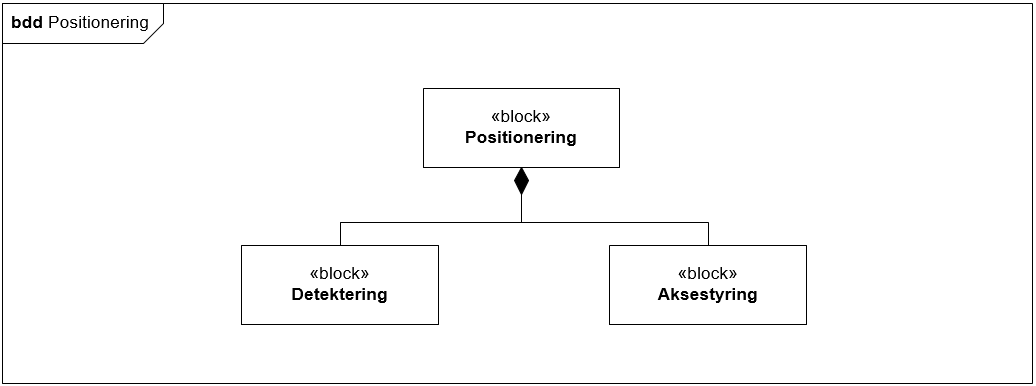
\includegraphics[scale=0.4]{Diagrammer/BDD_Positionering.png}}
	\caption{BDD over Positionering}
	\label{BDD_Positionering}
\end{figure}

\noindent\textbf{Detektering} består af sensorstyring som skal lokalisere flasken og dermed lade systemet kende flaskens koordinater.
\\
\\
\textbf{Aksestyring} driver \textbf{Detektering} langs flaskens akser.

\subsection{Åbningsmekanisme}
\begin{figure}[H]
	\centerline{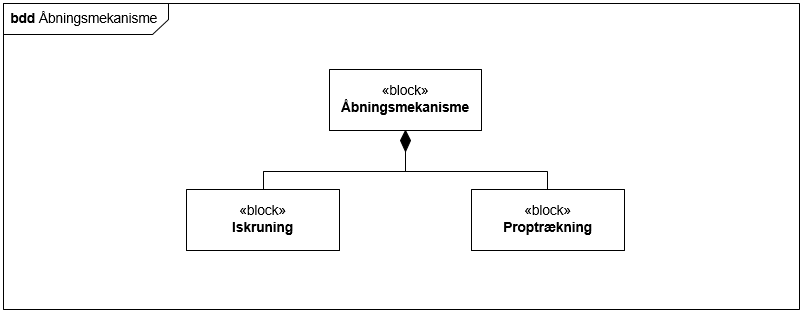
\includegraphics[scale=0.4]{Diagrammer/BDD_Aabningsmekanisme.png}}
	\caption{BDD over Åbningsmekanisme}
	\label{BDD_Aabningsmekanisme}
\end{figure}

\noindent\textbf{Iskruning} har ansvar for at iskrue i proppen.
\\
\\
\textbf{Proptrækning} har ansvar for at trække proppen ud af vinflasken.

\subsection{Allokeringsdiagram}
De blokke, der er opstillet på figur \ref{BDD_WinePrep}, allokeres på en række fysiske blokke, som vist på figur \ref{Allokering_WinePrep}.

\begin{figure}[H]
	\centerline{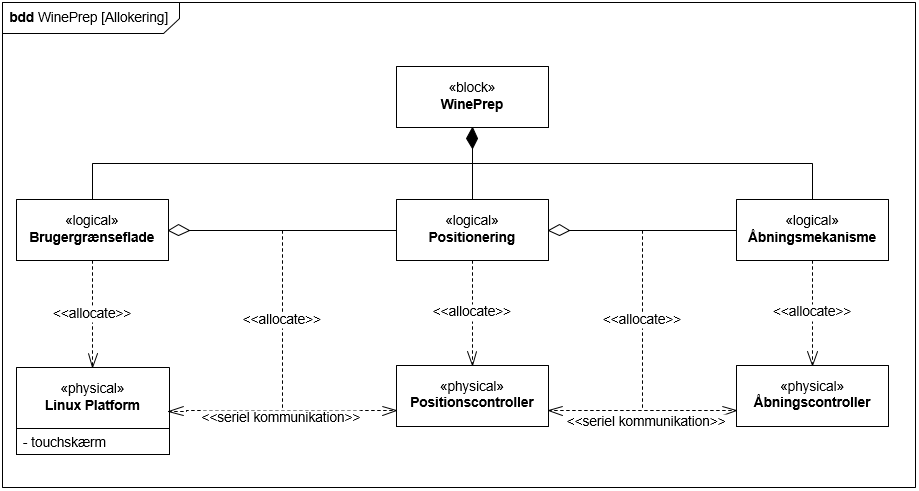
\includegraphics[scale=0.33]{tex/Arkitektur/Diagrammer/Allokering_WinePrep_to_MC}}
	\caption{Allokeringsdiagram over WinePrep}
	\label{Allokering_WinePrep}
\end{figure}

\noindent\textbf{Positionering} og \textbf{Åbningsmekanisme} er allokeret på hver deres microcontroller, som i dette projekt er besluttet til begge at være PSoC 5LP. \textbf{Brugergrænsefladen} er allokeret på en Linux-platform, som er DevKit8000.
\\
\\
\noindent Figur \ref{Allokering_WinePrep} viser ydermere allokeringen af det interne hierarki blandt blokkene. \textbf{Brugergrænsefladen} bruger \textbf{Positionering} vha. en seriel kommunikationsform. Det samme gør sig gældende mellem \textbf{Positionering} og \textbf{Åbningsmekanismen}.

\subsection{Endeligt BDD}
Figur \ref{BDD_WinePrepPDF} viser det endelige BDD over WinePrep. 

\begin{figure}[H]
	\centerline{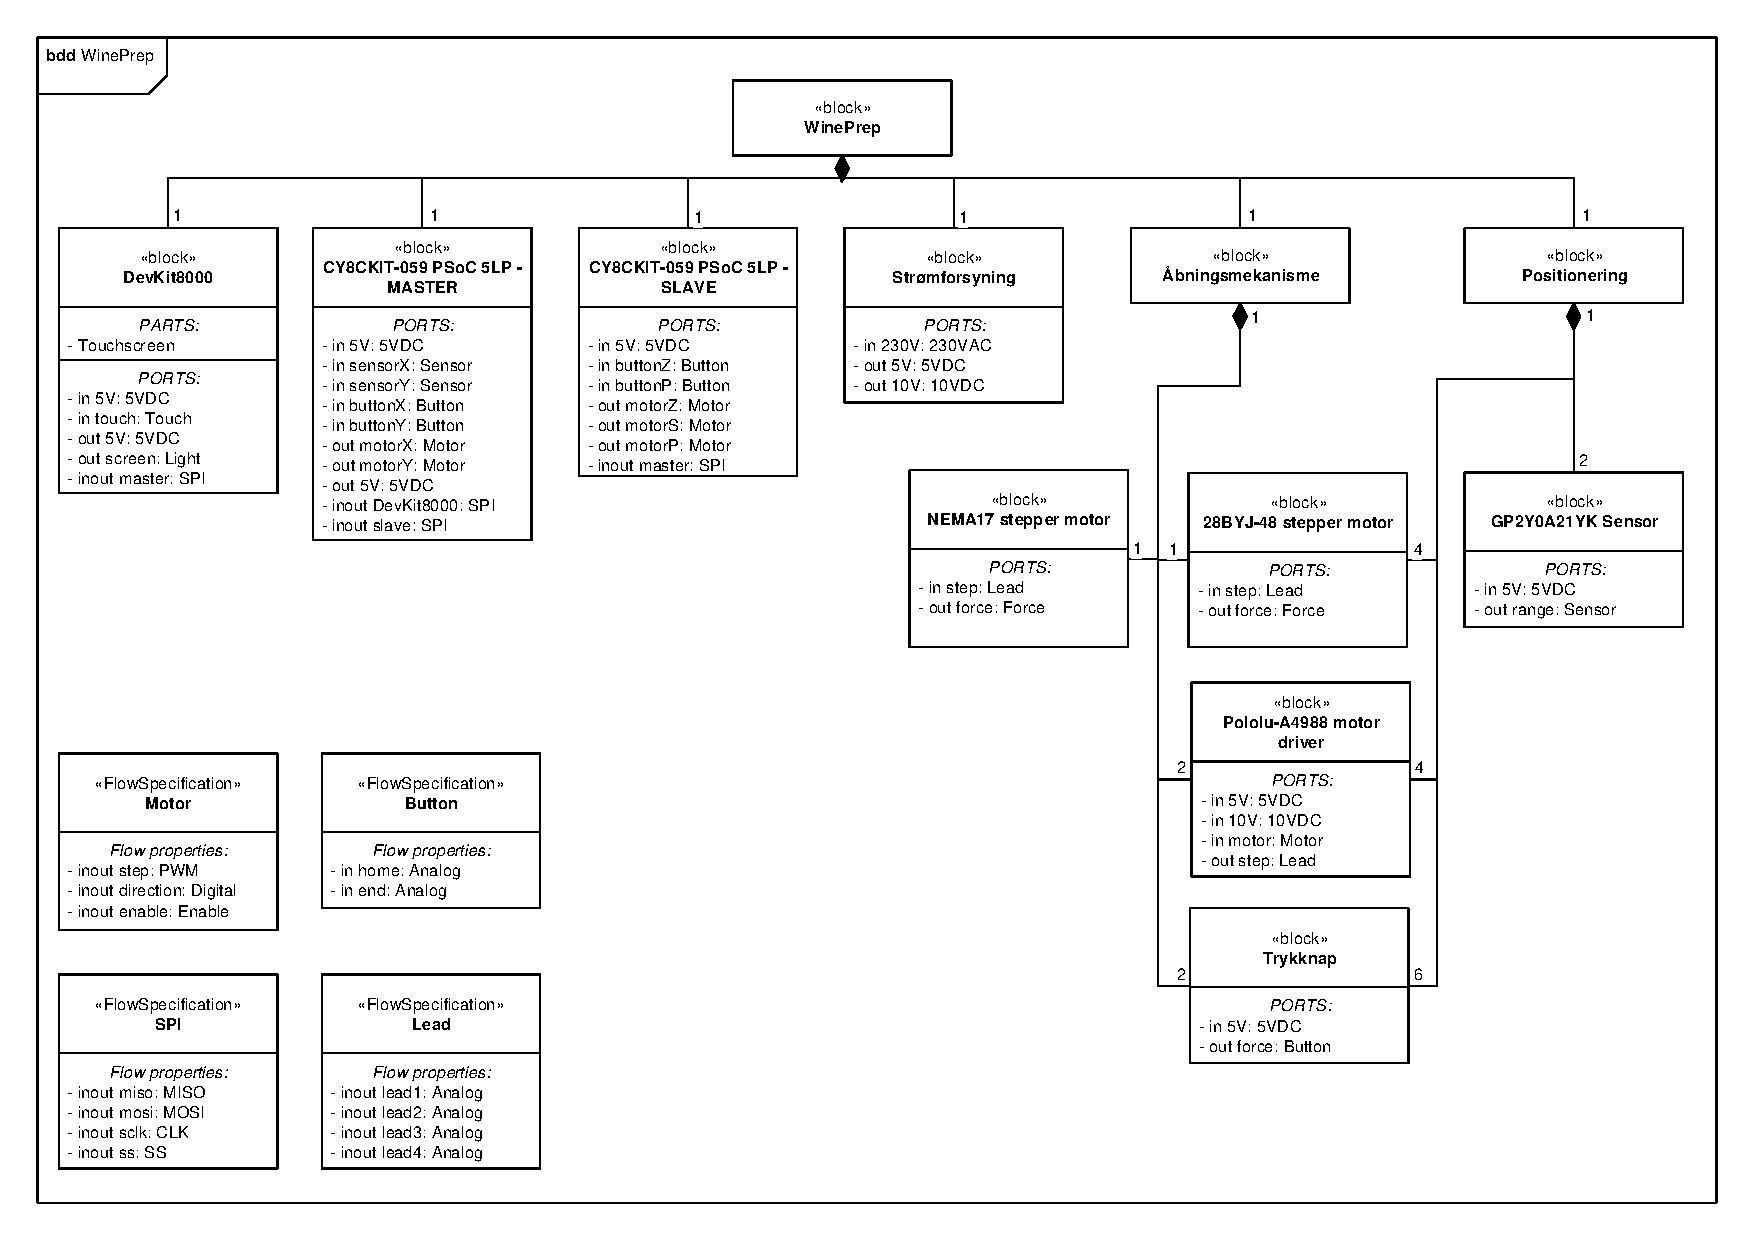
\includegraphics[scale=0.4]{Diagrammer/BDD_WinePrep.pdf}}
	\caption{BDD over WinePrep}
	\label{BDD_WinePrepPDF}
\end{figure}

